\documentclass[landscape]{article}
\usepackage[landscape,margin=0.7in]{geometry}
\usepackage{pgfplots}
\usepackage{tikz}
\usepackage{xcolor}
\pgfplotsset{compat=1.18}

\begin{document}
\pagestyle{empty}

\begin{figure}
    \centering
    \begin{tikzpicture}
        \begin{axis}[
            title={\Large Random Boarding Strategy - t = 110s},
            xlabel={Row Number},
            ylabel={Seat Position},
            xmin=19.5, xmax=39.5,
            ymin=0.5, ymax=6.5,
            ytick={1,2,3,4,5,6},
            yticklabels={A,B,C,D,E,F},
            xtick={20,22,24,26,28,30,32,34,36,38},
            width=\textwidth,
            height=0.27\textheight,
            colorbar=false,
            colormap={boarding}{
                color(0)=(white);
                color(0.33)=(yellow);
                color(0.66)=(orange);
                color(1)=(red)
            },
            point meta min=0,
            point meta max=1
        ]
            
        % Random boarding pattern - stage 1
        \addplot[matrix plot, mesh/rows=6, point meta=explicit] table [meta=C] {
            x y C
            20 1 1
            21 1 0
            22 1 0
            23 1 1
            24 1 0
            25 1 0
            26 1 1
            27 1 0
            28 1 0
            29 1 1
            30 1 0
            31 1 0
            32 1 1
            33 1 0
            34 1 0
            35 1 1
            36 1 0
            37 1 0
            38 1 1
            20 2 0
            21 2 1
            22 2 0
            23 2 0
            24 2 1
            25 2 0
            26 2 0
            27 2 1
            28 2 0
            29 2 0
            30 2 1
            31 2 0
            32 2 0
            33 2 1
            34 2 0
            35 2 0
            36 2 1
            37 2 0
            38 2 0
            20 3 0
            21 3 0
            22 3 1
            23 3 0
            24 3 0
            25 3 1
            26 3 0
            27 3 0
            28 3 1
            29 3 0
            30 3 0
            31 3 1
            32 3 0
            33 3 0
            34 3 1
            35 3 0
            36 3 0
            37 3 1
            38 3 0
            20 4 1
            21 4 0
            22 4 0
            23 4 1
            24 4 0
            25 4 0
            26 4 1
            27 4 0
            28 4 0
            29 4 1
            30 4 0
            31 4 0
            32 4 1
            33 4 0
            34 4 0
            35 4 1
            36 4 0
            37 4 0
            38 4 1
            20 5 0
            21 5 1
            22 5 0
            23 5 0
            24 5 1
            25 5 0
            26 5 0
            27 5 1
            28 5 0
            29 5 0
            30 5 1
            31 5 0
            32 5 0
            33 5 1
            34 5 0
            35 5 0
            36 5 1
            37 5 0
            38 5 0
            20 6 0
            21 6 0
            22 6 1
            23 6 0
            24 6 0
            25 6 1
            26 6 0
            27 6 0
            28 6 1
            29 6 0
            30 6 0
            31 6 1
            32 6 0
            33 6 0
            34 6 1
            35 6 0
            36 6 0
            37 6 1
            38 6 0
        };
        
        % Draw aisle line
        \draw[black, thick, dashed] (axis cs:19.5,3.5) -- (axis cs:39.5,3.5);
        
        % Legend
        \node[draw, fill=white, align=left, anchor=north west] at (axis cs:20,0) {
            \textbf{Status}\\
            \textcolor{white}{\rule{1em}{1em}} Empty\\
            \textcolor{yellow}{\rule{1em}{1em}} Boarding\\
            \textcolor{orange}{\rule{1em}{1em}} In process\\
            \textcolor{red}{\rule{1em}{1em}} Seated
        };
        
        % Description
        \node[draw, align=left, anchor=south west] at (axis cs:20,7) {
            \textbf{Random Boarding Strategy:}\\
            • Passengers board in random order without assigned groups\\
            • Leads to interference and seat conflicts in narrow aisles\\
            • No clear pattern emerges\\
            • Current status: Initial boarding phase (t = 110s)
        };
        \end{axis}
    \end{tikzpicture}
\end{figure}

\begin{figure}
    \centering
    \begin{tikzpicture}
        \begin{axis}[
            title={\Large Random Boarding Strategy - t = 220s},
            xlabel={Row Number},
            ylabel={Seat Position},
            xmin=19.5, xmax=39.5,
            ymin=0.5, ymax=6.5,
            ytick={1,2,3,4,5,6},
            yticklabels={A,B,C,D,E,F},
            xtick={20,22,24,26,28,30,32,34,36,38},
            width=\textwidth,
            height=0.27\textheight,
            colorbar=false,
            colormap={boarding}{
                color(0)=(white);
                color(0.33)=(yellow);
                color(0.66)=(orange);
                color(1)=(red)
            },
            point meta min=0,
            point meta max=1
        ]
            
        % Random boarding pattern - stage 2
        \addplot[matrix plot, mesh/rows=6, point meta=explicit] table [meta=C] {
            x y C
            20 1 1
            21 1 1
            22 1 1
            23 1 1
            24 1 0.33
            25 1 1
            26 1 1
            27 1 0.33
            28 1 1
            29 1 1
            30 1 0.33
            31 1 1
            32 1 1
            33 1 0.33
            34 1 1
            35 1 1
            36 1 0.33
            37 1 1
            38 1 1
            20 2 0.33
            21 2 1
            22 2 0.33
            23 2 1
            24 2 1
            25 2 0.33
            26 2 1
            27 2 1
            28 2 0.33
            29 2 1
            30 2 1
            31 2 0.33
            32 2 1
            33 2 1
            34 2 0.33
            35 2 1
            36 2 1
            37 2 0.33
            38 2 1
            20 3 1
            21 3 0
            22 3 1
            23 3 0.33
            24 3 1
            25 3 0
            26 3 1
            27 3 0.33
            28 3 1
            29 3 0
            30 3 1
            31 3 0.33
            32 3 1
            33 3 0
            34 3 1
            35 3 0.33
            36 3 1
            37 3 0
            38 3 1
            20 4 1
            21 4 0.33
            22 4 0
            23 4 1
            24 4 0.33
            25 4 0
            26 4 1
            27 4 0.33
            28 4 0
            29 4 1
            30 4 0.33
            31 4 0
            32 4 1
            33 4 0.33
            34 4 0
            35 4 1
            36 4 0.33
            37 4 0
            38 4 1
            20 5 0.33
            21 5 1
            22 5 0.33
            23 5 0.33
            24 5 1
            25 5 0.33
            26 5 0.33
            27 5 1
            28 5 0.33
            29 5 0.33
            30 5 1
            31 5 0.33
            32 5 0.33
            33 5 1
            34 5 0.33
            35 5 0.33
            36 5 1
            37 5 0.33
            38 5 0.33
            20 6 0
            21 6 0.33
            22 6 1
            23 6 0.33
            24 6 0
            25 6 0.33
            26 6 1
            27 6 0.33
            28 6 0
            29 6 0.33
            30 6 1
            31 6 0.33
            32 6 0
            33 6 0.33
            34 6 1
            35 6 0.33
            36 6 0
            37 6 0.33
            38 6 1
        };
        
        % Draw aisle line
        \draw[black, thick, dashed] (axis cs:19.5,3.5) -- (axis cs:39.5,3.5);
        
        % Legend
        \node[draw, fill=white, align=left, anchor=north west] at (axis cs:20,0) {
            \textbf{Status}\\
            \textcolor{white}{\rule{1em}{1em}} Empty\\
            \textcolor{yellow}{\rule{1em}{1em}} Boarding\\
            \textcolor{orange}{\rule{1em}{1em}} In process\\
            \textcolor{red}{\rule{1em}{1em}} Seated
        };
        
        % Description
        \node[draw, align=left, anchor=south west] at (axis cs:20,7) {
            \textbf{Random Boarding Strategy:}\\
            • Random filling pattern continues\\
            • Congestion occurs as multiple passengers attempt to reach their seats\\
            • Aisle blockages and seat interferences increase boarding time\\
            • Current status: Middle boarding phase (t = 220s)
        };
        \end{axis}
    \end{tikzpicture}
\end{figure}

\begin{figure}
    \centering
    \begin{tikzpicture}
        \begin{axis}[
            title={\Large Random Boarding Strategy - t = 330s},
            xlabel={Row Number},
            ylabel={Seat Position},
            xmin=19.5, xmax=39.5,
            ymin=0.5, ymax=6.5,
            ytick={1,2,3,4,5,6},
            yticklabels={A,B,C,D,E,F},
            xtick={20,22,24,26,28,30,32,34,36,38},
            width=\textwidth,
            height=0.27\textheight,
            colorbar=false,
            colormap={boarding}{
                color(0)=(white);
                color(0.33)=(yellow);
                color(0.66)=(orange);
                color(1)=(red)
            },
            point meta min=0,
            point meta max=1
        ]
            
        % Random boarding pattern - stage 3
        \addplot[matrix plot, mesh/rows=6, point meta=explicit] table [meta=C] {
            x y C
            20 1 1
            21 1 1
            22 1 1
            23 1 1
            24 1 1
            25 1 1
            26 1 1
            27 1 1
            28 1 1
            29 1 1
            30 1 1
            31 1 1
            32 1 1
            33 1 1
            34 1 1
            35 1 1
            36 1 1
            37 1 1
            38 1 1
            20 2 1
            21 2 1
            22 2 1
            23 2 1
            24 2 1
            25 2 1
            26 2 1
            27 2 1
            28 2 1
            29 2 1
            30 2 1
            31 2 1
            32 2 1
            33 2 1
            34 2 1
            35 2 1
            36 2 1
            37 2 1
            38 2 1
            20 3 1
            21 3 0.33
            22 3 1
            23 3 1
            24 3 1
            25 3 0.33
            26 3 1
            27 3 1
            28 3 1
            29 3 0.33
            30 3 1
            31 3 1
            32 3 1
            33 3 0.33
            34 3 1
            35 3 1
            36 3 1
            37 3 0.33
            38 3 1
            20 4 1
            21 4 1
            22 4 0.33
            23 4 1
            24 4 1
            25 4 0.33
            26 4 1
            27 4 1
            28 4 0.33
            29 4 1
            30 4 1
            31 4 0.33
            32 4 1
            33 4 1
            34 4 0.33
            35 4 1
            36 4 1
            37 4 0.33
            38 4 1
            20 5 1
            21 5 1
            22 5 1
            23 5 1
            24 5 1
            25 5 1
            26 5 1
            27 5 1
            28 5 1
            29 5 1
            30 5 1
            31 5 1
            32 5 1
            33 5 1
            34 5 1
            35 5 1
            36 5 1
            37 5 1
            38 5 1
            20 6 0.33
            21 6 1
            22 6 1
            23 6 1
            24 6 0.33
            25 6 1
            26 6 1
            27 6 1
            28 6 0.33
            29 6 1
            30 6 1
            31 6 1
            32 6 0.33
            33 6 1
            34 6 1
            35 6 1
            36 6 0.33
            37 6 1
            38 6 1
        };
        
        % Draw aisle line
        \draw[black, thick, dashed] (axis cs:19.5,3.5) -- (axis cs:39.5,3.5);
        
        % Legend
        \node[draw, fill=white, align=left, anchor=north west] at (axis cs:20,0) {
            \textbf{Status}\\
            \textcolor{white}{\rule{1em}{1em}} Empty\\
            \textcolor{yellow}{\rule{1em}{1em}} Boarding\\
            \textcolor{orange}{\rule{1em}{1em}} In process\\
            \textcolor{red}{\rule{1em}{1em}} Seated
        };
        
        % Description
        \node[draw, align=left, anchor=south west] at (axis cs:20,7) {
            \textbf{Random Boarding Strategy:}\\
            • Most seats filled in an inefficient pattern\\
            • Final passengers still struggling with seating conflicts\\
            • Late phase shows high seat occupancy but remaining passengers face delays\\
            • Estimated total boarding time: 18.7 minutes (t = 330s)
        };
        \end{axis}
    \end{tikzpicture}
\end{figure}

\end{document}